\documentclass{pre-tfg}

\usepackage{listings}
\usepackage{formular}
\usepackage[pdftex]{graphicx}
\usepackage[toc,page]{appendix}

\showhelp  % comenta o borra para eliminar ayudas

\title{ClassifiAds: Sistema de clasificación de páginas web con respecto a Banners}
\author{Alberto Aranda García y Cristian Gómez Portes}
\advisorFirst{Luis Rodríguez Benitez}
\advisorDepartment{Departamento de Tecnologías y Sistemas de Información}
\advisorSecond{}
\intensification{COMPUTACIÓN}
\docdate{2017}{Enero}


\DeclareGraphicsExtensions{.pdf,.png,.jpg}

\usepackage{color}
\definecolor{gray97}{gray}{.97}
\definecolor{gray75}{gray}{.75}
\definecolor{gray45}{gray}{.45}
\definecolor{dkgreen}{rgb}{0,0.6,0}
\definecolor{gray}{rgb}{0.5,0.5,0.5}
\definecolor{mauve}{rgb}{0.58,0,0.82}
\definecolor{light-gray}{gray}{0.25}
\definecolor{amber}{rgb}{1.0, 0.75, 0.0}
\definecolor{bostonuniversityred}{rgb}{0.8, 0.0, 0.0}

\lstset{ frame=Ltb,
     framerule=0pt,
     aboveskip=0.5cm,
     framextopmargin=3pt,
     framexbottommargin=3pt,
     framexleftmargin=0.4cm,
     framesep=0pt,
     rulesep=.4pt,
     backgroundcolor=\color{gray97},
     rulesepcolor=\color{black},
     %
     stringstyle=\ttfamily,
     showstringspaces = false,
     basicstyle=\small\ttfamily,
     commentstyle=\color{gray45},
     keywordstyle=\bfseries,
     %
     numbers=left,
     numbersep=15pt,
     numberstyle=\tiny,
     numberfirstline = false,
     breaklines=true,
   }

% minimizar fragmentado de listados
\lstnewenvironment{listing}[1][]
   {\lstset{#1}\pagebreak[0]}{\pagebreak[0]}

\lstdefinestyle{consola}
   {basicstyle=\scriptsize\bf\ttfamily,
    backgroundcolor=\color{gray75},
   }

% lenguaje que se utilizará
\lstdefinestyle{java}{
  language=Java,
  aboveskip=3mm,
  belowskip=3mm,
  showstringspaces=false,
  columns=flexible,
  basicstyle={\footnotesize\ttfamily},
  numberstyle={\tiny},
  numbers=left,
  keywordstyle=\color{blue},
  commentstyle=\color{dkgreen},
  stringstyle=\color{mauve},
  breaklines=true,
  breakatwhitespace=true,
  tabsize=3
}

\lstdefinestyle{makefile}
{
    numberblanklines=false,
    language=make,
    tabsize=4,
    keywordstyle=\color{red},
    identifierstyle= %plain identifiers for make
}

\renewcommand{\lstlistlistingname}{Índice de listado de código}

\begin{document}

\maketitle
\tableofcontents
\pagebreak
\listoffigures
\pagebreak
\lstlistoflistings

\newpage

\section{OBJETIVOS}

El presente proyecto trata de clasificar con un sistema multi-agente ciertas páginas con respecto al número de anuncios o ``banners'' y sus tipos (contenido publicitario, sexual, etc.) asociadas a éstas.

El sistema multiagente contará con cuatro agentes, los cuales recogerán información de diferentes páginas (los anuncios o ``banners'' que encuentre) para enviárselo a otro agente, que estará en una capa inferior. Éste se encargará de procesar esa información para establecer el ranking y comprobar de qué tipo son los anuncios. Una vez tengamos la información procesada, ésta será enviada a otro agente, en una capa más inferior, que será el encargado de mostrar el ranking a el usuario mediante una interfaz o similar.

Con respecto a la tecnología a utilizar, se usará Java como lenguaje de programación y Jade, un marco de software que simplifica la implementación de sistemas multi-agentes en Java -- en \cite{bellifemine2002jade} se puede encontrar más información sobre esta plataforma. Además, se utilizarán las siguientes librerías para facilitar el desarrollo del proyecto:

\begin{itemize}
 \item \textit{Jsoup}: librería utilizada para trabajar con HTML. Sitio de descarga: \url{https://jsoup.org/download}.
\item  \textit{Regex}: librería para trabajar con expresiones regulares. Viene incluida en el paquete ``util'' de Java.
\end{itemize}

\section{ESTRUCTURA DEL SMA}
El sistema multiagente desarrollado se compone de seis agentes como se especificó en el apartado anterior. Los cuatro agentes de la capa superior contarán con un comportamiento, el cual dedicará su tiempo a buscar diferentes tipos de anuncios. En el caso de que no se encontrará ningún anuncio, el comportamiento volvería a iniciarse para rastrear otra página diferente.

Una vez el agente haya encontrado la información requerida (todos los links de la página), éste lo enviará a una capa inferior donde se aloja el agente de procesamiento. Este agente tendrá cuatro comportamientos, los cuales se encargarán de procesar la información que cada agente de la capa superior le envió. El procesamiento constará de comparar los links recibidos con los dominios de anuncios alojados en un archivo llamado ``blacklist''. Además, el agente de procesamiento responderá a cada agente enviándole una respuesta de confirmación de recepción de los datos para que éstos mueran.

El agente de procesamiento gestionará la información que le envíe cada agente en el orden en el que éstos lo hagan. Después de que toda la información haya sido procesada, éste lo enviará al agente interfaz, el cual se encargará de la visualización de los datos.

Finalmente, después de que los datos hayan sido mostrados, el usuario podra abortar la ejecución del programa cuando éste lo desee. Acto seguido, el agente interfaz morirá.

En la Figura \ref{fig:flujo-sma} se puede ver el flujo que los agentes seguirán a lo largo de la ejecución.

\begin{figure}[h]
    \centering
    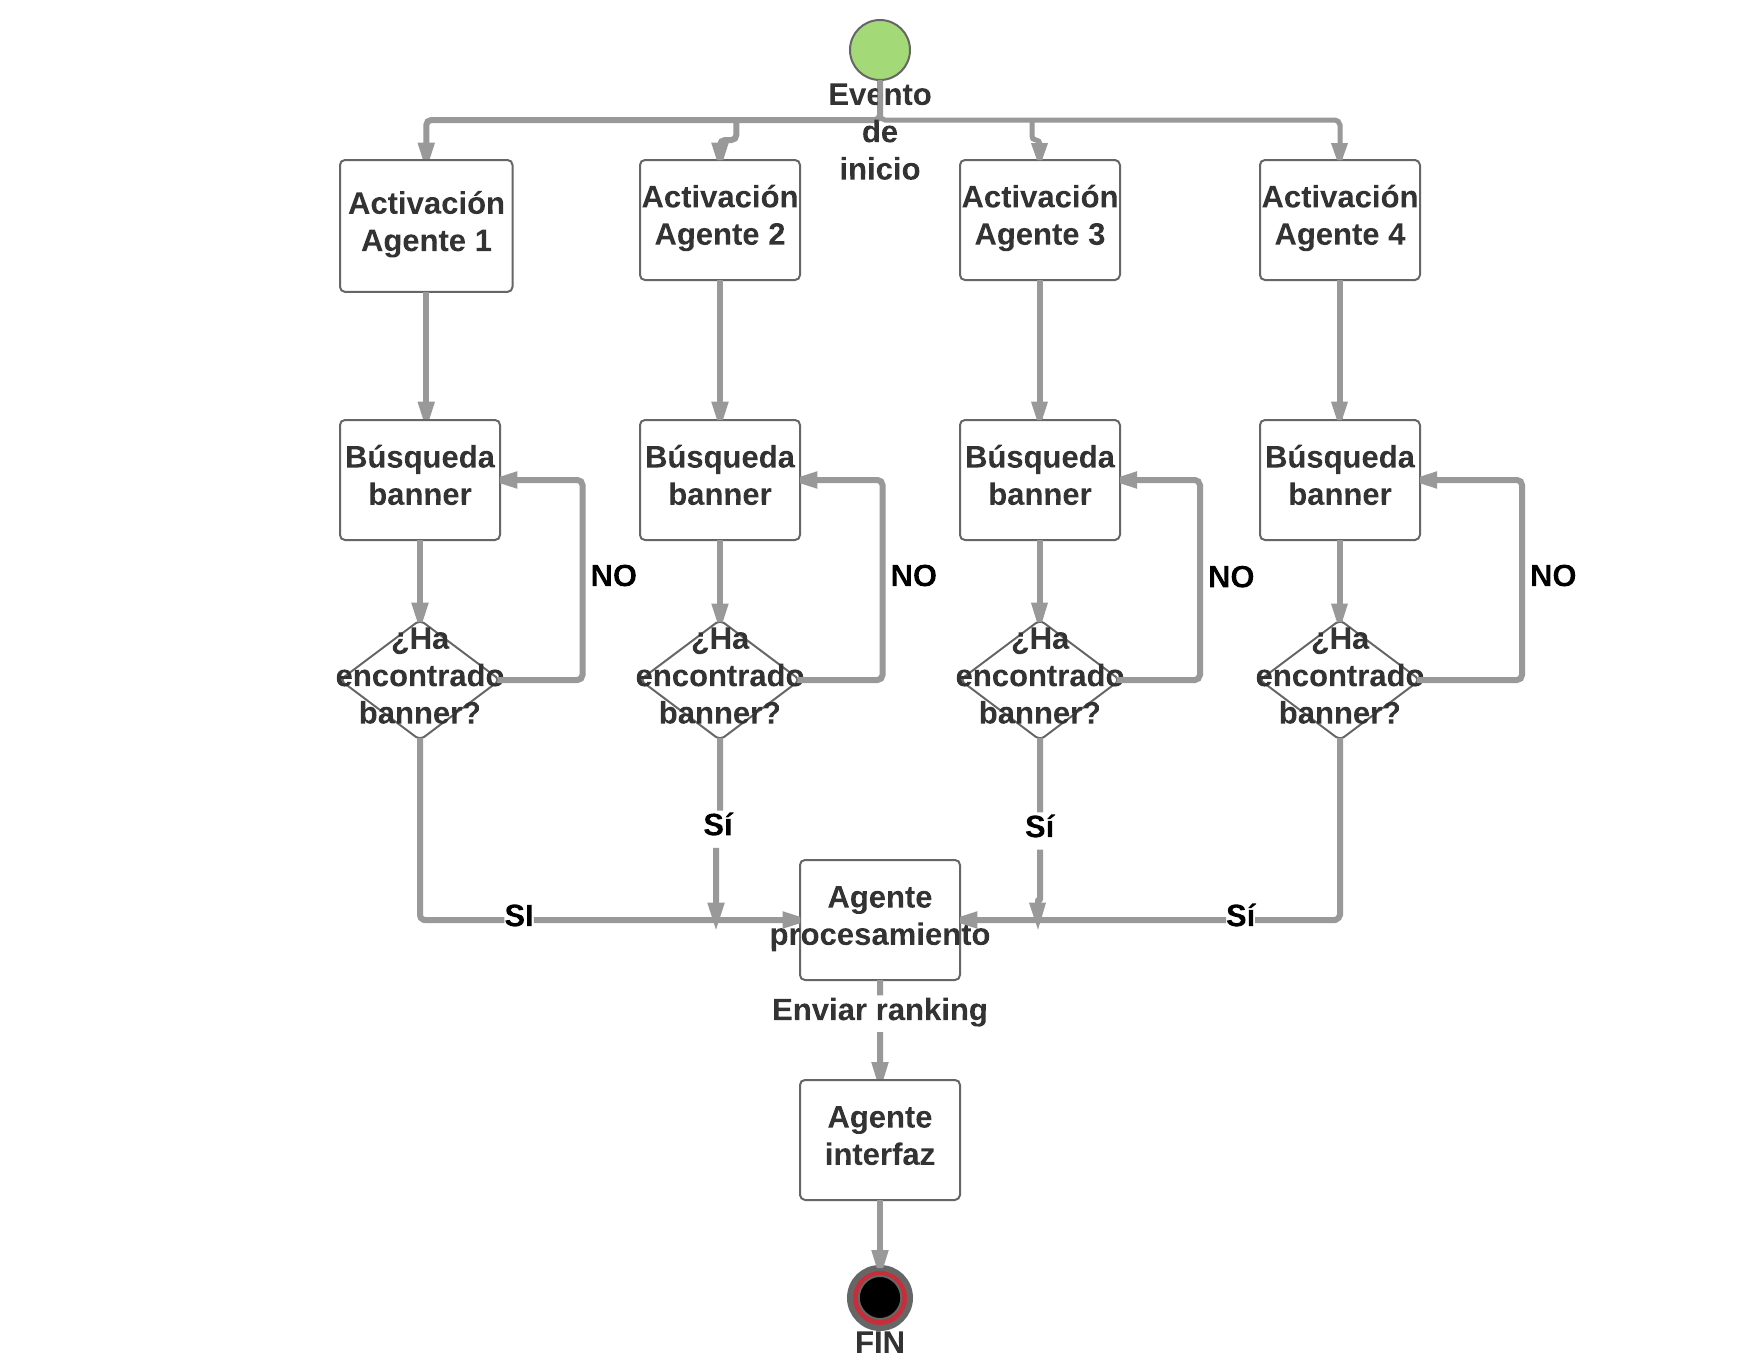
\includegraphics[width=1.0\textwidth]{flujo-sma}
    \caption{Diagrama de flujo del sistema multi-agente}
    \label{fig:flujo-sma}
\end{figure}

\clearpage

\section{MEDIOS QUE SE HAN UTILIZADO}
En el presente apartado se pretenden describir todos los medios que se utilizarán para llevar a cabo el proyecto
expuesto en este trabajo. Por un lado, se especificarán los medios hardware que se prevén necesarios para el desarrollo
del sistema. Por otro lado, se detallarán los medios software (lenguaje, entorno de desarrollo, herramientas de gestion y 
planificación, etc.) que se requieren para la construcción del presente proyecto.

\subsection{MEDIOS HARDWARE}
Para el desarrollo del sistema se ha requerido de dos equipos con sistemas \textit{Windows} y \textit{Linux}, dado
que los integrantes del grupo cuentan con ambos sistemas respectivamente. En cuanto a las especificaciones, ambos equipos
cuentan con unas caracterísitcas habituales por lo general, ya que no es necesario de un computador potente para el despliegue y desarrollo del
proyecto.

\subsection{MEDIOS SOFTWARE}

\begin{itemize}
 \item \textbf{Lenguaje}: para el desarrollo del sistema se ha utilizado el lenguaje Java, ya que la plataforma para el desarrollo 
 de agentes que se utilizará para la construcción del presente proyecto está implementada con el mismo.
 \item \textbf{Edición de código}: para la edición de código se ha utilizado el entorno \textit{Eclipse}, el cual facilita la escritura 
 del código debido al resaltado sintáctico que incorpora para el lenguaje Java.
 \item \textbf{Entorno de desarrollo}: el entorno a utilizar ha sido \textit{Eclipse}, debido a la facilidad mediante \textbf{JARs} de 
 integrar la plataforma para el desarrollo de agentes \textbf{JADE}, además del potente depurador que incorpora para ayudar a 
 corregir fallos en el código.
 \item \textbf{Orgnización}: se ha utilizado \textit{Git} como sistema de control de versiones y \textit{GitHub} como sistema web
 para la gestión de código. La elección de ambos sistemas se debe a la experiencia adquirida a lo largo de los últimos años de grado
 para el desarrollo de prácticas en diferentes asignaturas.
 \item \textbf{Documentación}: la documentación a desarrollar se ha hecho mediante el sistema de elaboración de textos \LaTeX.
\end{itemize}

\section{EJECUCIÓN DEL SISTEMA}

Basándonos en la configuración de la máquina virtual proporcionada para el desarrollo de las prácticas de la asignatura de Sistemas Multi-Agentes, 
se ha procedido a la construcción de un \textit{Makefile} para automatizar todo el proceso de compilación y ejecución
del sistema.

En primer lugar, deberemos copiar la carpeta del proyecto dentro de la carpeta de \textit{jade} y posicionarnos en la raiz del proyecto ClassifiAds, 
donde se encuentra el archivo que automatiza los procesos mencionados anteriormente. Para compilar todos los archivos \verb|.java| tendremos 
que ejecutar el siguiente comando: \textbf{make compile}. Este comando generará todos los \verb|.class| de los archivos fuente y los moverá a la
carpeta \textit{classes}, la cual usará Jade para ejecutar el sistema.

En segundo y último lugar, se procederá a ejecutar el comando que despliega el sistema expuesto en este trabajo. El comando es el siguiente:
\textbf{make run}. Este comando hace las llamadas pertinentes a Jade y ejecuta en un orden establecido los receptores y emisores del sistema
para que la comunicación entre ellos sea la correcta. En el siguiente listado se puede ver una parte del código que automatiza los procesos de compilación y 
ejecución, además de los parámetros de los que hacemos uso para el correcto funcionamiento de la aplicación.

\begin{lstlisting}[caption=Makefile,style=makefile]

PARAMS 			= 	"printer:presentation.PrinterAgent("processor");\
			processor:domain.ProcessorAgent("retriever1", "retriever2", "retriever3", "retriever4")\
			;retriever1:domain.RetrieverAgent("www.as.com");retriever2:domain.RetrieverAgent("www.sports.es")\
			;retriever3:domain.RetrieverAgent("www.mundodeportivo.com")\
			;retriever4:domain.RetrieverAgent("www.marca.com")" 

compile:
	$(JC) $(JFLAGS) $(SRC1)/*.java $(SRC2)/*.java

run:
	$(JVM) -cp $(CLASSPATH) $(JADE) $(PARAMS)

\end{lstlisting}

\newpage

%%%%%%%%%%%%%%%%%%%%% ANEXOS %%%%%%%%%%%%%%%%%%%%%%%%%%%%%%%%%
\appendix
\section{CODIGO}

En el siguiente anexo se plasma el código que se ha desarrollado para la implementación del sistema multi-agente. Además,
se pretende explicar alguna de las partes que se consideran importantes para mejorar la comprensión del código y justificar
el porqué de su uso.

\subsection{RetrieverAgent.java}

Este clase genera un agente que se encarga de recoger los links de una página web.

\begin{lstlisting}[caption=Código de recuperación de links de una URL,style=java]

/**
 * Agent that retrieves links from web
 */
package domain;

/* imports of jade */
import jade.core.AID;
import jade.core.Agent;
import jade.core.behaviours.Behaviour;
import jade.lang.acl.MessageTemplate;
import jade.lang.acl.ACLMessage;

/* imports of jsoup */
import org.jsoup.Jsoup;
import org.jsoup.nodes.Document;
import org.jsoup.nodes.Element;
import org.jsoup.select.Elements;

import java.io.IOException;
import java.util.ArrayList;
import java.util.regex.Matcher;
import java.util.regex.Pattern;

/**
 * @author Alberto Aranda Garcia y Cristian Gomez Portes
 *
 */

public class RetrieverAgent extends Agent{
	private Object[] args;

	protected void setup() {
		/* Get arguments */
		args = getArguments();

		/* check arguments */
		if(args != null && args.length == 1) {

			/* Get the url */
			String url = "http://" + (String) args[0] + "/";

			/* Add behaviour */
			addBehaviour(new RetrievalBehaviour(url));
		}
		else
			System.out.println("Error. You must type an url as an argument");
	}

	private class RetrievalBehaviour extends Behaviour{
		private String url;
		private boolean end;
		private MessageTemplate template = null;

		/**
		 * Constructor of the RetrievalBehaviour class
		 * @param url
		 */
		public RetrievalBehaviour(String url) {
			this.url = url;

			AID aid = new AID();
			aid.setLocalName("processor");

			/* Return a template from message that matches with 'Processor' */
			MessageTemplate senderFilter = MessageTemplate.MatchSender(aid);

			/* Return a template from message that matches with this performative */
			MessageTemplate informFilter = MessageTemplate.MatchPerformative(ACLMessage.INFORM);

			/* Build template */
			template = MessageTemplate.and(senderFilter, informFilter);

		}

		/**
		 * Initialization of the variables
		 */
		public void onStart() {
			end = false;
		}

		/**
		 * Run the process of the behaviour
		 */
		public void action() {
			print("Fetching %s...", url);
			
			/* pattern to obtain only the domain */
			String pattern = "((?:[a-z][a-z\\.\\d\\-]+)\\.(?:[a-z][a-z\\-]+))(?![\\w\\.])";
			
			Pattern r = Pattern.compile(pattern);

			Document doc = null;
			try {
				doc = Jsoup.connect(url).get();
			} catch (IOException e) {
				System.out.println(e.getMessage());
			}
			Elements links = doc.select("a[href]");
			ArrayList<String> attributes = new ArrayList<String>();

			/* Retrieve links */
			print("\nLinks: (%d) from <%s>", links.size(), url);
			for (Element link : links) {
				String attr = link.attr("abs:href");
	            Matcher m = r.matcher(attr);
	            if(m.find())
	            	attributes.add(m.group(0));
			}
			
			/* Store the web page and links */
			Storage storage = new Storage(attributes, url);

			/* Prepare message */
			AID aid = new AID();
			aid.setLocalName("processor");

			/* Send message if we have found links */
			if(links.size() > 0) {
				ACLMessage sendMessage = new ACLMessage(ACLMessage.INFORM);
				sendMessage.setSender(getAID());
				sendMessage.addReceiver(aid);
				try {
					sendMessage.setContentObject(storage);
					send(sendMessage);
				} catch (IOException e) {
					// TODO Auto-generated catch block
					e.printStackTrace();
				}

				/* Block behaviour until message is received */
				blockingReceive(template);
				end = true;
			}
		}

		/**
		 * Print message in a predetermine format
		 * @param msg
		 * @param args
		 */
		private void print(String msg, Object... args) {
			System.out.println(String.format(msg, args));
		}

		/**
		 * Behaviour finalizes if end is equal to true
		 */
		public boolean done() {
			return end;
		}

		/**
		 * Kill the agent
		 */
		public int onEnd() {
			doDelete();
			return 0;
		}
	}

	/**
	 * Free resources from the agent
	 */
	protected void takeDown() {
		System.out.println(getLocalName() + " frees resources");
	}
}

\end{lstlisting}

En esta clase se hace uso de expresiones regulares porque queremos obtener el dominio de la url, es decir, queremos eliminar
la parte reservada para http o https y la continuación de .com .es o similar. Por ejemplo, si recibimos la siguiente url:
https://www.loquesea.com/sdfmvdf0wew4t5/34t obtendremos mediante la expresión regular lo siguiente:
www.loquesea.com. Esto nos permite agilizar el proceso de búsqueda de anuncios, ya que el archivo `ad\_servers.txt`
contiene dominios de este estilo.

\subsection{ProcessorAgent.java}

Este clase genera un agente que se encarga de procesar los links que recibe del agente anterior para extraer los anuncios.

\begin{lstlisting}[caption=Código de extracción de anuncios de varios links de una URL,style=java]

/**
 * Agent that processes information from RetrieverAgent
 */
package domain;

/* imports of jade */
import jade.core.AID;
import jade.core.Agent;
import jade.core.behaviours.Behaviour;
import jade.core.behaviours.ParallelBehaviour;
import jade.lang.acl.MessageTemplate;
import jade.lang.acl.UnreadableException;
import jade.lang.acl.ACLMessage;

import java.io.IOException;
import java.util.ArrayList;

/**
 * @author Alberto Aranda Garcia y Cristian Gomez Portes
 *
 */

public class ProcessorAgent extends Agent{
	private Object[] args;

	protected void setup() {
		/* Get arguments */
		args = getArguments();

		/* check arguments */
		if(args != null && args.length == 4) {
			/* Create ParallelBehaviour */
			ParallelBehaviour pb = new ParallelBehaviour(ParallelBehaviour.WHEN_ALL) {
				/**
				 * Kill the Agent
				 */
				public int onEnd() {
					doDelete();
					return super.onEnd();
				}
			};

			/* Get retriever */
			for(Object retriever : args) {
				/* Add subBehaviour */
				pb.addSubBehaviour(new ProcessorBehaviour((String) retriever));

			}
			
			/* Add ParallelBehaviour */
			addBehaviour(pb);
		}
		else
			System.out.println("Error. You must type the name of agent as an argument");
	}
	private class ProcessorBehaviour extends Behaviour{
		private String agent;
		private boolean end;
		private MessageTemplate template = null;

		/**
		 * Constructor of the ProcessalBehaviour class
		 * @param agent
		 */
		public ProcessorBehaviour(String agent) {
			this.agent = agent;

			AID aid = new AID();
			aid.setLocalName(agent);

			/* Return a template from message that matches with 'Processor' */
			MessageTemplate senderFilter = MessageTemplate.MatchSender(aid);

			/* Return a template from message that matches with this performative */
			MessageTemplate informFilter = MessageTemplate.MatchPerformative(ACLMessage.INFORM);

			/* Build template */
			template = MessageTemplate.and(senderFilter, informFilter);
		}

		/**
		 * Initialization of the variables
		 */
		public void onStart() {
			end = false;
		}

		/**
		 * Run the process of the behaviour
		 */
		public void action() {
			ACLMessage message = receive(template);
			if(message != null) {
				Storage storage = null;
				ArrayList<String> links = null;
				String webpage = null;
				try {
					storage = (Storage) message.getContentObject();
					print("Message received from %s", agent);

					/* get web page */
					webpage = storage.getWebpage();

					/* get links */
					links = storage.getLinks();

					/* object that contains all ad servers */
					ServerList serverlist = new ServerList();

					/* ArrayList that will contain the ad links */
					ArrayList<String> adlinks = new ArrayList<String>();

					/* Process links and compare them with the serverlist */
					for(String link : links) {
						if(serverlist.contains(link)) {
							adlinks.add(link);
						}
					}					
					print("Ads detected in %s: %s", webpage, adlinks.size());

					/* Store the web page and ad links */
					Storage storage_ads = new Storage(adlinks, webpage);

					/* Prepare message */
					AID aid = new AID();
					aid.setLocalName("printer");

					ACLMessage sendMessage = new ACLMessage(ACLMessage.INFORM);
					sendMessage.setSender(getAID());
					sendMessage.addReceiver(aid);

					sendMessage.setContentObject(storage_ads);
					send(sendMessage);

				} catch (UnreadableException e) {
					// TODO Auto-generated catch block
					e.printStackTrace();
				} catch (IOException e) {
					// TODO Auto-generated catch block
					e.printStackTrace();
				}

				/* Prepare message */
				AID aid = new AID();
				aid.setLocalName(agent);

				/* Send response */
				ACLMessage response = message.createReply();
				response.setSender(getAID());
				response.addReceiver(aid);

				send(response);
				end = true;
			}else {
				/* Block the agent */
				block();
			}
		}

		/**
		 * Print message in a predetermine format
		 * @param msg
		 * @param args
		 */
		private void print(String msg, Object... args) {
			System.out.println(String.format(msg, args));
		}

		/**
		 * Behaviour finalizes if end is equal to true
		 */
		public boolean done() {
			return end;
		}
	}

	/**
	 * Free resources from the agent
	 */
	protected void takeDown() {
		System.out.println(getLocalName() + " frees resources");
	}
}

\end{lstlisting}

\subsection{ServerList.java}

Esta clase se encarga de leer el archivo `ad\_servers.txt` para almacenar todos los dominios de anuncios que nos podemos encontrar
en diferentes páginas web.

\begin{lstlisting}[caption=Código de lectura e inserción de dominios de anuncios,style=java]

/**
 * Store all ad links into an ArrayList
 */
package domain;

import java.io.File;
import java.io.FileNotFoundException;
import java.util.HashSet;
import java.util.Scanner;

/**
 * @author Alberto Aranda Garcia y Cristian Gomez Portes
 *
 */
public class ServerList {
	private HashSet<String> serverList;
	
	/**
	 * Constructor of the ServerList class
	 */
	public ServerList(){
		this.serverList = read_ad_servers_file("ad_servers.txt");
	}
	
	/**
	 * Get serverList
	 * @return
	 */
	public HashSet<String> getServerList(){
		return serverList;
	}
	
	/**
	 * Set serverList
	 * @param serverList
	 */
	public void setServerList(HashSet<String> serverList) {
		this.serverList = serverList;
	}
	
	/**
	 * Whether the serverList contains or not a given server
	 * @param server
	 * @return
	 */
	public boolean contains(String server) {
		return serverList.contains(server);
	}
	
	/**
	 * Read file that contains all ad servers
	 * @param path
	 * @return
	 */
	private HashSet<String> read_ad_servers_file(String path){
		Scanner s =  null;
		try {
			s = new Scanner(new File(path));
		} catch (FileNotFoundException e) {
			// TODO Auto-generated catch block
			e.printStackTrace();
		}
		HashSet<String> list = new HashSet<String>();
		while (s.hasNextLine()){
		    list.add(s.next());
		}
		s.close();
		
		return list;
	}
}

\end{lstlisting}

\subsection{Storage.java}

Esta clase es la encargada de almacenar todos los links recuperados por el \textit{RetrieverAgent.java} y asociarlos a la página web
de donde fueron extraídos.

\begin{lstlisting}[caption=Código que almacena los links junto a la página web de donde fueron recuperados,style=java]

/**
 * Store the web page and the ad links which are related to it
 */
package domain;

import java.io.Serializable;
import java.util.ArrayList;

/**
 * @author Alberto Aranda Garcia y Cristian Gomez Portes
 *
 */
public class Storage implements Serializable{
	private ArrayList<String> links;
	private String webpage;
	
	/**
	 * Constructor of the Storage class
	 * @param links
	 * @param webpage
	 */
	public Storage(ArrayList<String>links, String webpage) {
		this.links = links;
		this.webpage = webpage;
	}
	
	/**
	 * Get links
	 * @return
	 */
	public ArrayList<String> getLinks() {
		return links;
	}
	
	/**
	 * Set links
	 * @param links
	 */
	public void setLinks(ArrayList<String> links) {
		this.links = links;
	}
	
	/**
	 * Get web page
	 * @return
	 */
	public String getWebpage() {
		return webpage;
	}
	
	/**
	 * Set web page
	 * @param webpage
	 */
	public void setWebpage(String webpage) {
		this.webpage = webpage;
	}
	
}

\end{lstlisting}

\subsection{PrinterAgent.java}

Esta clase genera un agente que se encarga de pintar la información que recibe del \textit{ProcessorAgent.java} en forma de tabla.

\begin{lstlisting}[caption=Código que pinta el número de anuncios encontrados en una página en forma de tabla,style=java]

/**
 * Agent that prints the information that has received from ProcessoAgent
 */
package presentation;

import java.util.ArrayList;
import java.util.Collection;
import java.util.Enumeration;
import java.util.Hashtable;

import domain.Storage;
import jade.core.AID;
import jade.core.Agent;
import jade.core.behaviours.Behaviour;
import jade.lang.acl.ACLMessage;
import jade.lang.acl.MessageTemplate;
import jade.lang.acl.UnreadableException;

/**
 * @author Alberto Aranda Garcia y Cristian Gomez Portes
 *
 */
public class PrinterAgent extends Agent{
	private Object[] args;
	private Hashtable<String, Integer> table;
	
	protected void setup() {
		table = new Hashtable<String, Integer>();
		
		/* Get arguments */
		args = getArguments();

		/* check arguments */
		if(args != null && args.length == 1) {
			
			/* Get the agent */
			String agent = (String) args[0];

			/* Add behaviour */
			addBehaviour(new PrinterBehaviour(agent));
		}
		else
			System.out.println("Error. You must type the name of agent as an argument");
	}
	
	private class PrinterBehaviour extends Behaviour {
		private String agent;
		private boolean end;
		private int messageReceived;
		private MessageTemplate template = null;
		
		/**
		 * Constructor of the ProcessalBehaviour class
		 * @param agent
		 */
		public PrinterBehaviour(String agent) {
			this.agent = agent;
			
			AID aid = new AID();
			aid.setLocalName(agent);

			/* Return a template from message that matches with 'Processor' */
			MessageTemplate senderFilter = MessageTemplate.MatchSender(aid);

			/* Return a template from message that matches with this performative */
			MessageTemplate informFilter = MessageTemplate.MatchPerformative(ACLMessage.INFORM);

			/* Build template */
			template = MessageTemplate.and(senderFilter, informFilter);
		}
		
		/**
		 * Initialization of the variables
		 */
		public void onStart() {
			end = false;
			messageReceived = 0;
		}
		
		/**
		 * Run the process of the behaviour
		 */
		public void action() {
			if(messageReceived <= 3) {
				ACLMessage message = receive(template);
				if(message != null) {
					messageReceived++;
					Storage storage = null;
					ArrayList<String> ads = null;
					String webpage = null;
					try {
						storage = (Storage) message.getContentObject();
						print("Message received from %s", agent);

						/* get web page */
						webpage = storage.getWebpage();

						/* get ads */
						ads = storage.getLinks();
						
						/* Add information in table */
						table.put(webpage, ads.size());
						
					} catch (UnreadableException e) {
						// TODO Auto-generated catch block
						e.printStackTrace();
					}
				}else {
					/* Block the agent */
					block();
				}
			}else {
				/* Print solution */
				print("******************** %s *********************", "Solution");
				String leftAlignFormat = "| %-40s | %-4d |%n";
				System.out.format("+------------------------------------------+------+%n");
				System.out.format("| WebPage                                  | Ads  |%n");
				System.out.format("+------------------------------------------+------+%n");
				Enumeration<String> keys = table.keys();
				do {
					String key = keys.nextElement();
					int value = table.get(key);
				    System.out.format(leftAlignFormat, key, value);
				}while(keys.hasMoreElements());
				System.out.format("+------------------------------------------+------+%n");
				end = true;
			}
		}
		
		/**
		 * Print message in a predetermine format
		 * @param msg
		 * @param args
		 */
		private void print(String msg, Object... args) {
			System.out.println(String.format(msg, args));
		}
		
		/**
		 * Behaviour finalizes if end is equal to true
		 */
		public boolean done() {
			return end;
		}
		
		public int onEnd() {
			doDelete();
			return 0;
		}
	}
	
	/**
	 * Free resources from the agent
	 */
	protected void takeDown() {
		System.out.println(getLocalName() + " frees resources");
	}
}

\end{lstlisting}

\subsection{Makefile}

Este código es el encargado de automatizar las tareas de compilación y ejecución.

\begin{lstlisting}[caption=Código que automatiza la tarea de compilación y ejecución,style=makefile]

#!/usr/bin/make -f
# -*- mode:makefile -*-

JC 			= javac
JVM			= java
CLASSPATH		:= "$(CLASSPATH):lib/jsoup-1.10.3.jar"
CLASSDIR 		= ../classes
JFLAGS 			= -d $(CLASSDIR) -cp $(CLASSPATH)
JADE 			= jade.Boot -agents
PARAMS 			= 	"printer:presentation.PrinterAgent("processor");\
			processor:domain.ProcessorAgent("retriever1", "retriever2", "retriever3", "retriever4")\
			;retriever1:domain.RetrieverAgent("www.as.com");retriever2:domain.RetrieverAgent("www.sports.es")\
			;retriever3:domain.RetrieverAgent("www.mundodeportivo.com")\
			;retriever4:domain.RetrieverAgent("www.marca.com")" 
SRC1 			= src/domain
SRC2			= src/presentation

compile:
	$(JC) $(JFLAGS) $(SRC1)/*.java $(SRC2)/*.java

run:
	$(JVM) -cp $(CLASSPATH) $(JADE) $(PARAMS)

clean:
	$(RM) $(CLASSES)/domain/*.class $(CLASSES)/presentation/*.class

\end{lstlisting}

\clearpage

\bibliographystyle{alpha}
\singlespacing
\bibliography{ejemplo}

\end{document}

% Local Variables:
% coding: utf-8
% mode: flyspell
% ispell-local-dictionary: "castellano8"
% mode: latex
% End:
